
\begin{figure}
	\floatbox{figure}[\FBwidth]
	{
		\caption{Gender differences in readability, by \textit{JEL} classification}\label{figure1}
	}
	{
		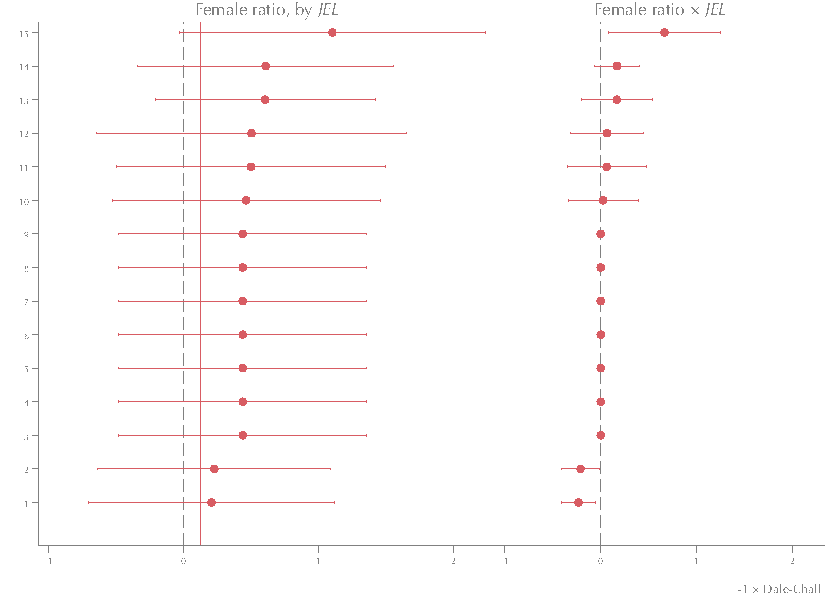
\includegraphics[width=12.3cm]{$HOME/Dropbox/Readability/draft/pdf/figure1.pdf}
		\floatfoot{
			\begin{minipage}{1.0\linewidth}
				\setlength{\belowdisplayskip}{2pt}
				\setlength{\belowdisplayshortskip}{0pt}
				\setlength{\abovedisplayskip}{2pt}
				\setlength{\abovedisplayshortskip}{0pt}
				\tiny\textit{Notes}. Sample 5,777 articles, including 561 from \textit{AER Papers \& Proceedings} (see~\autoref{footnote34}). Codes A, B, M and P dropped due to small sample sizes of female-authored papers (see~\autoref{footnote33}). Estimates from an OLS regression of:
				$$R_j=\,\beta_0+\beta_1\text{female ratio}_j + \bm\upbeta_2\,\vect J_j + \bm\upbeta_3\,\text{female ratio}_j\times\vect J_j + \bm\uptheta\,\vect X_j + \vep_j,$$
				where $R_j$ is the readability score for article $j$; $\text{female ratio}_j$ is paper $j$'s ratio of female authors to total authors; $\vect J_j$ is a $15\times1$ column vector with $k$th entry a binary variable equal to one if article $j$ is classified as the $k$th \textit{JEL} code; $\vect X_j$ is a vector of editor, journal, year, institution, English language dummies and quality controls (citation count and \(\text{max. }T_j\) fixed effects); $\vep_j$ is the error term. Left-hand graph shows marginal effects of female ratio for each \textit{JEL} code ($\beta_1+\beta_3^k$); the pink vertical line is the mean effect at observed \textit{JEL} codes (0.129, standard error 0.046). Right-hand graph displays interaction terms ($\beta_3^k$). Horizontal lines represent 90 percent confidence intervals from standard errors adjusted for clustering on editor.
			\end{minipage}
		}
	}
\end{figure}